\section{Medical QA Implementation Details and Additional Results}
\label{app:medical_qa}

This appendix provides implementation details for our medical question-answering experiments, connecting the general conformal risk control framework to the specific problem of controlling LLM factuality. We describe the problem setup and notation (Section~\ref{subsec:medqa_setup}), prior approaches to conformal factuality (Section~\ref{subsec:medqa_prior_approaches}), loss functions for factuality control including the non-monotonic FDR loss (Section~\ref{subsec:medqa_loss_functions}), experimental setup (Section~\ref{subsec:medqa_experimental_setup}), and hyperparameters (Section~\ref{subsec:medqa_hyperparams}).

\subsection{Problem Setup and Notation}
\label{subsec:medqa_setup}

Following \citet{mohri2024language} and \citet{cherian2024large}, we formalize the natural language factuality setting as follows. Each data sample $Z_i$ is a prompt-response-claim-annotation tuple:
\begin{align}
    Z_i := (X_i, X_i', \boldsymbol{C}_i, \boldsymbol{Y}_i),
\end{align}
where $X_i$ is the prompt (question), $X_i'$ is the full LLM response, $\boldsymbol{C}_i = (C_{i1}, \ldots, C_{ik_i})$ is the vector of atomic subclaims extracted from $X_i'$, and $\boldsymbol{Y}_i = (Y_{i1}, \ldots, Y_{ik_i})$ contains binary annotations indicating whether each subclaim is factually correct ($Y_{ij} = 1$) or incorrect ($Y_{ij} = 0$).

For each subclaim $C_{ij}$, let $p(C_{ij} \mid X_i) \in [0, 1]$ denote a prompt-conditional confidence score estimating the likelihood that the subclaim is factual. Higher scores indicate greater confidence in factuality.

\subsection{Prior Approaches to Conformal Factuality}
\label{subsec:medqa_prior_approaches}

\paragraph{Mohri \& Hashimoto (2024).} \citet{mohri2024language} achieve conformal factuality guarantees by filtering subclaims based on a threshold $\tau$ determined by split conformal prediction. A subclaim $C_{ij}$ is included in the filtered response if $p(C_{ij} \mid X_i) \geq \tau$. The corresponding non-conformity score for each response is the smallest threshold such that all included subclaims are factual:
\begin{align}
    s(Z_i) = \inf\big\{\tau : Y_{ij} = 1 \ \text{for all} \ j \ \text{with} \ p(C_{ij} \mid X_i) \geq \tau \big\}.
\end{align}
The threshold $\hat{\tau}$ is then selected as the $(1-\alpha)$-quantile of the calibration scores:
\begin{align}
    \hat{\tau} = \inf \Big\{\tau : \frac{1}{n}\sum_{i=1}^n\mathbbm{1}\{s(Z_i) \leq \tau\} \geq \frac{\lceil(n+1)(1-\alpha)\rceil}{n}\Big\}.
\end{align}

\paragraph{Cherian et al.\ (2024).} \citet{cherian2024large} extend this approach using conditional calibration and multicalibration to provide guarantees that hold across different subgroups of prompts, addressing the limitation that marginal guarantees may not hold uniformly across topics or question types.

\subsection{Loss Functions for Factuality Control}
\label{subsec:medqa_loss_functions}

\paragraph{Binary indicator loss (prior work).} The loss function implicitly used by \citet{mohri2024language} and \citet{cherian2024large} is the binary indicator for whether any included subclaim is incorrect:
\begin{align}
    L_i^{\text{binary}}(\tau) = \mathbbm{1}\Big\{\exists \ j : p(C_{ij} \mid X_i) \geq \tau \ \text{and} \ Y_{ij} = 0\Big\}.
\end{align}
Controlling this loss at level $\alpha$ guarantees $\mathbb{P}(\text{any included claim is false}) \leq \alpha$. This loss is monotonically non-increasing in $\tau$ by construction: as the threshold increases, fewer claims are included, so the probability of including a false claim can only decrease.

\paragraph{False discovery rate loss (this work).} We instead use a more granular loss: the false discovery rate (FDR), \textit{i.e.}, the fraction of included subclaims that are false:
\begin{align}
    L_i(\tau) = \underbrace{\frac{\sum_{j=1}^{k_i} (1 - Y_{ij}) \cdot \mathbbm{1}\{p(C_{ij} \mid X_i) \geq \tau\}}{\sum_{j=1}^{k_i} \mathbbm{1}\{p(C_{ij} \mid X_i) \geq \tau\}}}_{\text{FDR}_i(\tau) = 1 - \text{Precision}_i(\tau)},
    \label{eq:fdr_loss}
\end{align}
with $L_i(\tau) = 0$ when no claims are included. This is precisely $1 - \text{Precision}_i(\tau)$, where precision is the fraction of included claims that are true. Controlling this loss at level $\alpha$ ensures:
\begin{align}
    \mathbb{E}[\text{FDR}_i(\tau)] \leq \alpha \quad \Longleftrightarrow \quad \mathbb{E}[\text{Precision}_i(\tau)] \geq 1 - \alpha.
\end{align}

\paragraph{Why FDR control requires generalized CRC.} Unlike the binary loss, the FDR loss in \eqref{eq:fdr_loss} is not monotonic in $\tau$. As $\tau$ increases, both the numerator (false claims included) and denominator (total claims included) decrease, but not necessarily at the same rate. This non-monotonicity means standard CRC \citep{angelopoulos2022conformal} does not apply directly, motivating our generalized CRC approach.

For methods requiring monotonicity, one can use the monotonized loss:
\begin{align}
    \tilde{L}_i(\tau) = \sup_{\tau' \geq \tau} L_i(\tau'),
\end{align}
which upper-bounds the FDR and is monotonically non-increasing by construction. However, this monotonization can be overly conservative.

\paragraph{Reward metric: true claim recall.} While we control the FDR (our loss), we measure the recall of true claims as our reward metric:
\begin{align}
    \text{Recall}_i(\tau) = \frac{\sum_{j: Y_{ij} = 1} \mathbbm{1}\{p(C_{ij} \mid X_i) \geq \tau\}}{\sum_{j=1}^{k_i} Y_{ij}},
    \label{eq:recall_metric}
\end{align}
\textit{i.e.}, the fraction of true subclaims that are retained after filtering. For a given FDR target $\alpha$, methods that achieve higher recall preserve more useful information while satisfying the same safety constraint.

\subsection{Experimental Setup}
\label{subsec:medqa_experimental_setup}

Our experimental setup closely follows \citet{cherian2024large}, with the key modification of controlling the FDR loss \eqref{eq:fdr_loss} and measuring recall \eqref{eq:recall_metric} as a reward metric.

\subsubsection{Dataset}

We use the \textbf{MedLFQA} (Medical Long-Form Question Answering) dataset from \citet{jeong2024olaph}, which aggregates four established medical QA benchmarks:
\begin{itemize}
    \item \textbf{HealthSearchQA} ($n = 3047$): Consumer health questions
    \item \textbf{K-QA} ($n = 1077$): Knowledge-intensive medical questions, with a subset having gold-standard physician responses (K-QA Golden, $n = 201$) and the remainder having LLM-generated responses (K-QA Silver)
    \item \textbf{LiveQA} ($n = 100$): Real consumer health questions from the National Library of Medicine
    \item \textbf{MedicationQA} ($n = 627$): Questions about medications and drug interactions
\end{itemize}
Each prompt is accompanied by either an LLM or human-generated reference response, which serves as ground truth for evaluating factual accuracy.

\subsubsection{Data Generation Pipeline}

We use the annotated dataset from \citet{cherian2024large}, which was constructed through a three-stage pipeline:
\begin{enumerate}
    \item \textbf{Response generation}: GPT-3.5-Turbo was queried with each medical question to obtain a candidate response $X_i'$.
    \item \textbf{Subclaim extraction}: GPT-4o parsed each response into atomic subclaims $\boldsymbol{C}_i = (C_{i1}, \ldots, C_{ik_i})$.
    \item \textbf{Factuality annotation}: GPT-3.5-Turbo evaluated whether each subclaim is substantiated by the reference response, yielding binary annotations $Y_{ij} \in \{0, 1\}$.
\end{enumerate}
For subclaim scoring, we use \textbf{self-evaluation scores} $p(C_{ij} \mid X_i)$, where the LLM is prompted to assess its own confidence in each claim.

\subsubsection{Methods Compared}

We compare three conformal risk control methods:
\begin{itemize}
    \item \textbf{gCRC (proposed)}: Generalized conformal risk control as described in Section~\ref{sec:theory}, which searches thresholds from safest to most aggressive and stops when the augmented empirical risk exceeds $\alpha$.

    \item \textbf{Monotonized-losses CRC} \citep{angelopoulos2022conformal, mohri2024language}: Applies standard CRC to the monotonized loss $\tilde{L}_i(\tau) = \sup_{\tau' \geq \tau} L_i(\tau')$, which upper-bounds the FDR.

    \item \textbf{Learn Then Test (LTT)} \citep{angelopoulos2021learn}: A multiple testing approach using Hoeffding-Bentkus $p$-values to identify valid thresholds with family-wise error rate control. Unlike CRC methods, LTT does not add a conservative test-point loss term.
\end{itemize}

\subsubsection{Experimental Protocol}

\begin{itemize}
    \item \textbf{Calibration/test split}: 70\%/30\% random split of the dataset
    \item \textbf{Risk levels}: $\alpha \in \{0.005, 0.01, 0.015, \ldots, 0.10\}$ (20 values)
    \item \textbf{Threshold grid}: 200 candidate thresholds sampled from the empirical distribution of subclaim scores
    \item \textbf{Random seeds}: Results averaged over 10 independent train/test splits
    \item \textbf{Score jittering}: Uniform noise ($\sim 10^{-8}$) added to break ties
\end{itemize}

\subsection{Hyperparameters}
\label{subsec:medqa_hyperparams}

Table~\ref{tab:medqa_hyperparameters} summarizes the experimental configuration.

\begin{table}[h]
\centering
\caption{Hyperparameters for medical QA experiments.}
\label{tab:medqa_hyperparameters}
\begin{tabular}{lll}
\toprule
\textbf{Parameter} & \textbf{Symbol} & \textbf{Value} \\
\midrule
Calibration fraction & -- & 0.7 \\
Number of trials & -- & 10 \\
Threshold grid size & $|\Lambda|$ & 200 \\
Risk levels tested & $\alpha$ & $\{0.005, 0.01, \ldots, 0.10\}$ \\
Score jitter magnitude & -- & $10^{-8}$ \\
Response LLM & -- & GPT-3.5-Turbo \\
Subclaim extraction LLM & -- & GPT-4o \\
Annotation LLM & -- & GPT-3.5-Turbo \\
Subclaim scoring method & -- & Self-evaluation \\
\bottomrule
\end{tabular}
\end{table}


\subsection{Additional Medical QA Results}
\label{app:med_QA_add_results}


\begin{figure}[!t]
\centering
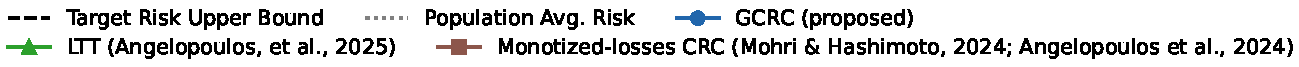
\includegraphics[width=\linewidth]{figures/legend_logprobs_risk.pdf}\\[0.5em]
\textbf{Log-Probabilities Subclaim Scoring}
\\
\begin{subfigure}{0.42\linewidth}
    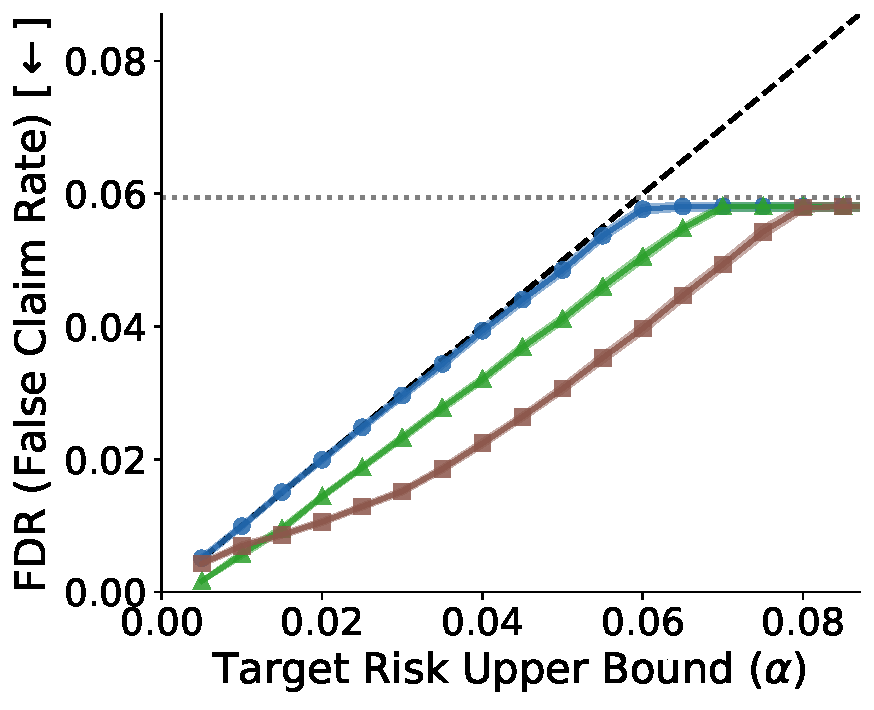
\includegraphics[width=\linewidth]{figures/loss_factuality_fdrLoss_logprobsScoring_risk_25trials_200ngrid.pdf}
\end{subfigure}
\hfill
\begin{subfigure}{0.42\linewidth}
    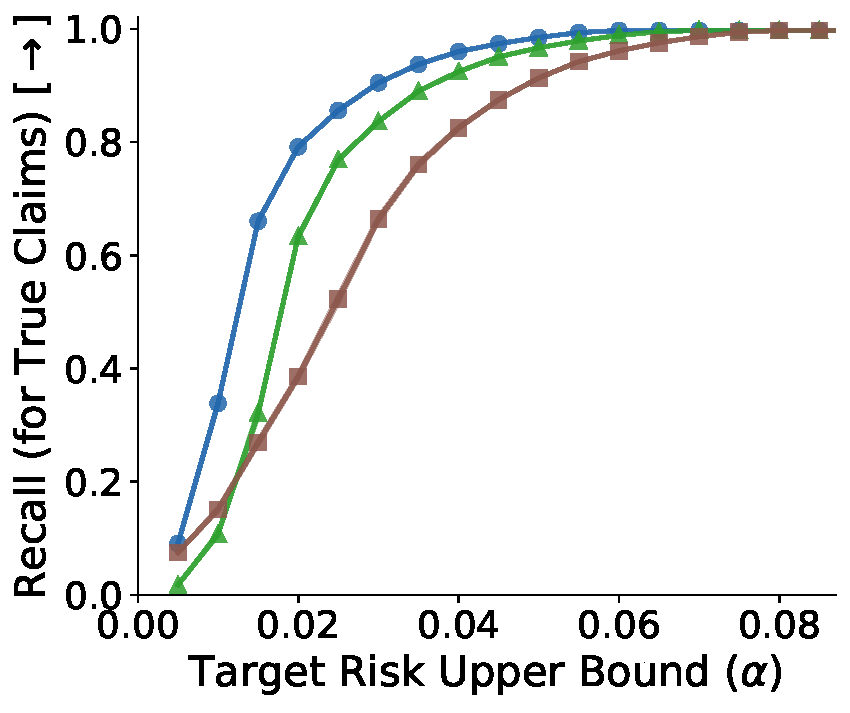
\includegraphics[width=\linewidth]{figures/loss_factuality_fdrLoss_logprobsScoring_claims_25trials_200ngrid.pdf}
\end{subfigure}
\\
\textbf{Self-Evaluation Subclaim Scoring}
\\
\begin{subfigure}{0.42\linewidth}
    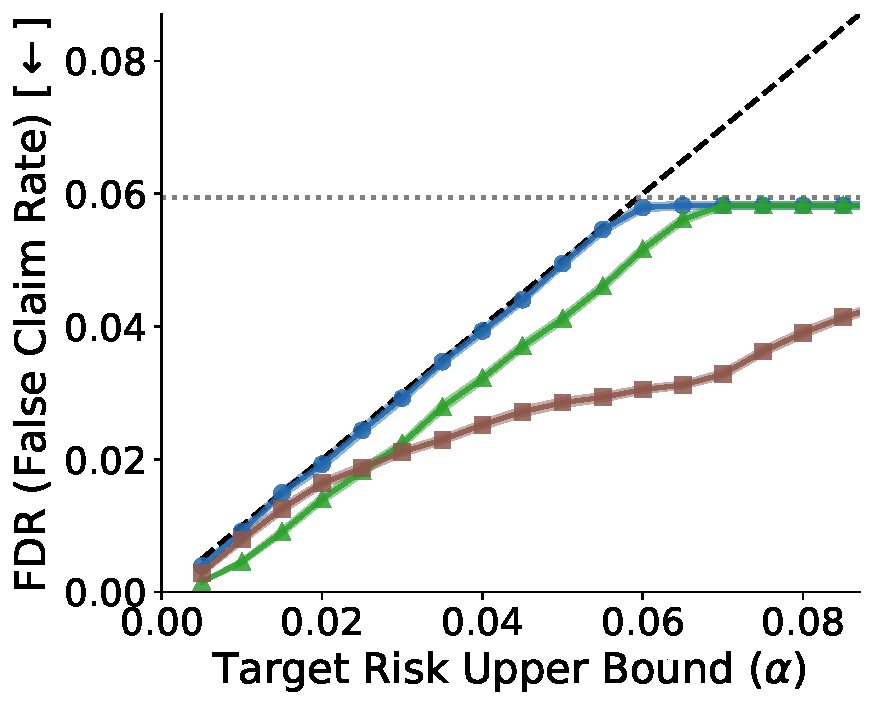
\includegraphics[width=\linewidth]{figures/loss_factuality_fdrLoss_selfevalsScoring_risk_25trials_200ngrid.pdf}
\end{subfigure}
\hfill
\begin{subfigure}{0.42\linewidth}
    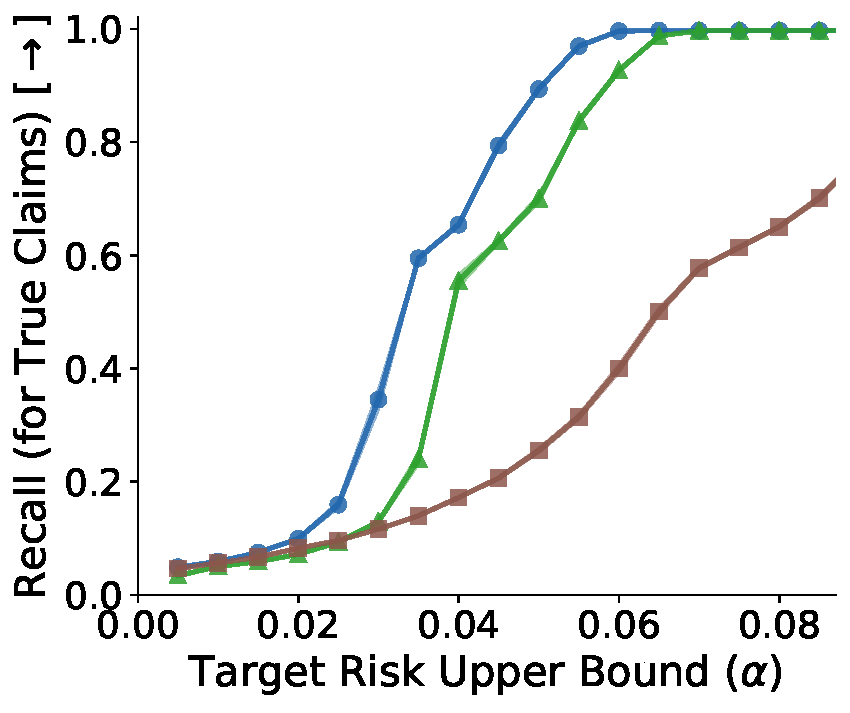
\includegraphics[width=\linewidth]{figures/loss_factuality_fdrLoss_selfevalsScoring_claims_25trials_200ngrid.pdf}
\end{subfigure}
\\
\textbf{Frequency Subclaim Scoring}
\\
\begin{subfigure}{0.42\linewidth}
    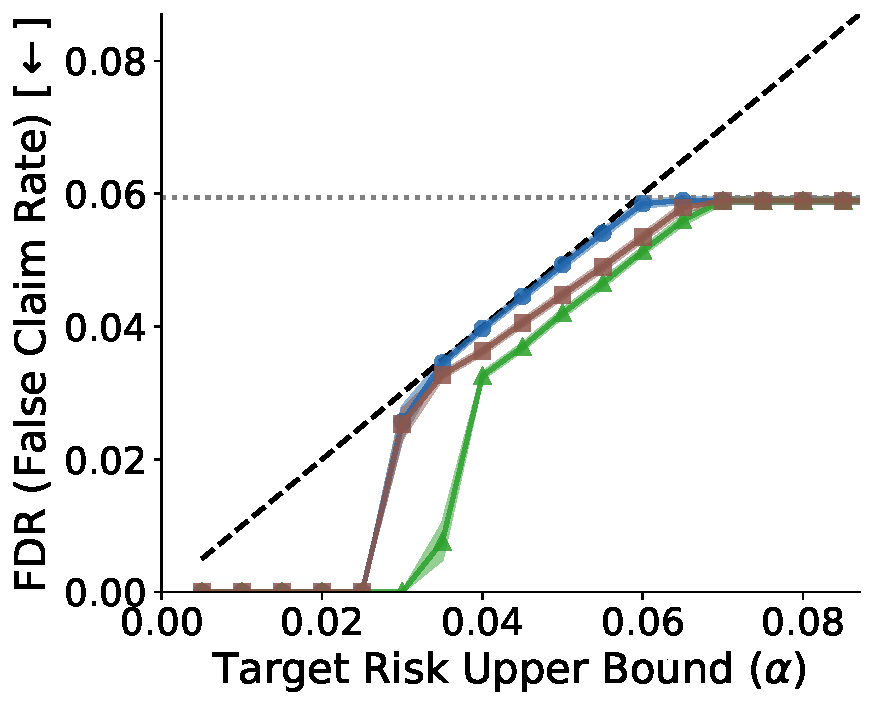
\includegraphics[width=\linewidth]{figures/loss_factuality_fdrLoss_frequencyScoring_risk_25trials_200ngrid.pdf}
\end{subfigure}
\hfill
\begin{subfigure}{0.42\linewidth}
    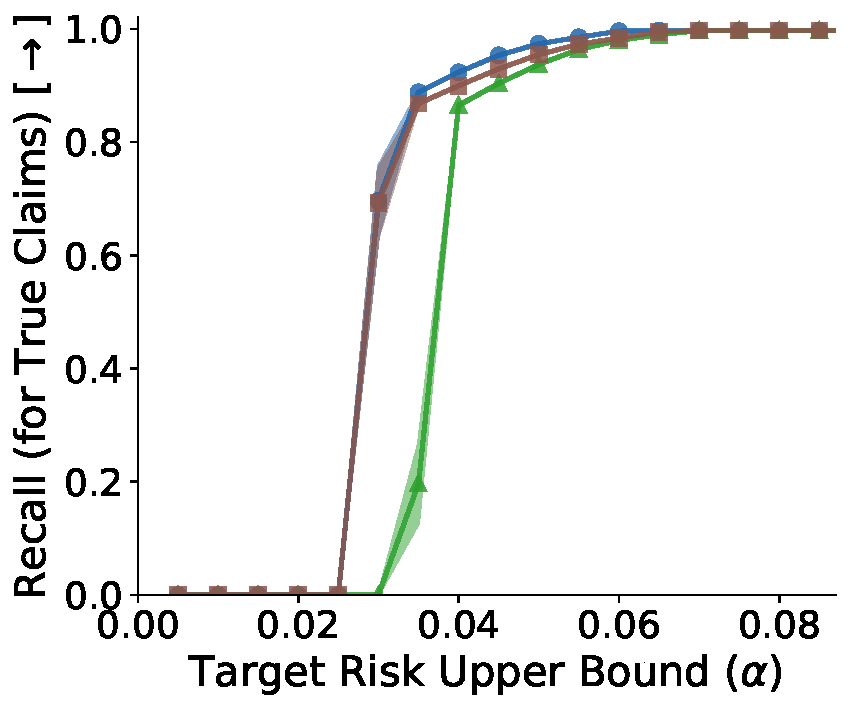
\includegraphics[width=\linewidth]{figures/loss_factuality_fdrLoss_frequencyScoring_claims_25trials_200ngrid.pdf}
\end{subfigure}
\caption{Medical QA factuality control results on MedLFQA on three subclaim scoring methods: log-probabilities \textbf{(top row)}, self-evaluation \textbf{(middle row)}, and frequency \textbf{(bottom row)}. \textbf{Left column:} Empirical FDR (fraction of retained claims that are false) vs.\ target risk level $\alpha$. The black dashed line indicates $y = x$; valid methods should fall at or below this line. \textbf{Right column:} Recall (fraction of true claims retained) vs.\ $\alpha$. gCRC tightly controls FDR at the target level while achieving superior recall to baselines. Results averaged over 25 random splits. Error regions are standard errors.}
\end{figure}

\clearpage
